\documentclass[tikz, convert={density=600,outext=.png}]{standalone}
\usepackage{tikz}
\usepackage{varwidth}
\usetikzlibrary{positioning}
\usetikzlibrary{arrows.meta,arrows}
\usetikzlibrary{backgrounds}

\begin{document}
\newcommand{\nnz}{{nnz}}

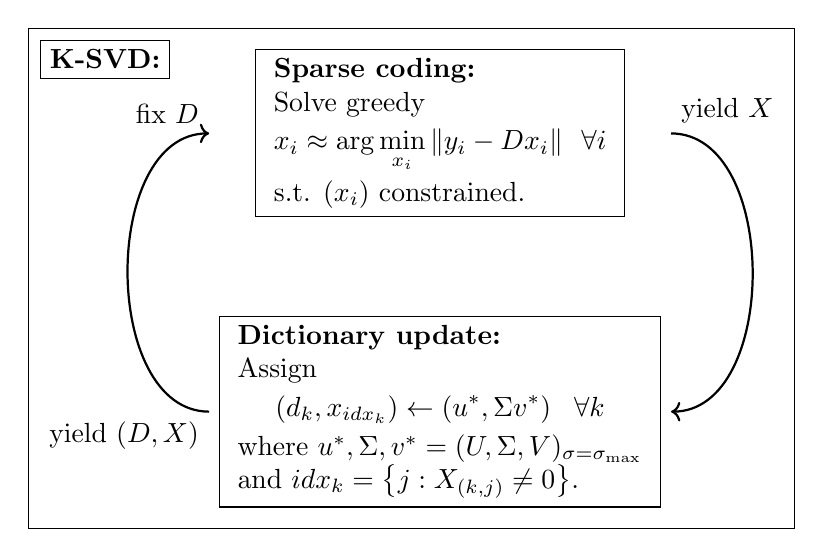
\begin{tikzpicture}[framed]

  \node (sparse-coding) {\framebox{
      {\begin{varwidth}{\linewidth}
          \textbf{Sparse coding:}\\
          Solve greedy\vspace{0.2em}
          \[
            x_i \approx \arg \min_{x_i} \|y_{i} - D x_{i}\| \ \ \forall i \vspace{-0.4em}
          \]
          s.t. \(\nnz(x_{i})\) constrained.
        \end{varwidth}}
    }};

  \node[below=of sparse-coding] (dictionary-update) {\framebox{
      \begin{varwidth}{\linewidth}
        \textbf{Dictionary update:}\\
        Assign \vspace{0.2em}
        \[
          \left(d_{k}, x_{{idx}_k}\right) \leftarrow \left( u^\ast, \Sigma v^\ast\right) \ \ \forall k \vspace{-0.4em}
        \]
        where \(u^\ast, \Sigma, v^\ast = (U, \Sigma, V)_{\sigma = \sigma_{\rm max}}\)\\
        and \({idx}_k = \left\{ j : X_{(k, j)} \neq 0 \right\}\).
      \end{varwidth}
    }};

  \draw[out=0, in=0, ->, thick] (sparse-coding.east -| dictionary-update.east) to node[pos=0.0, right, anchor=south west] {yield \(X\)} (dictionary-update);
  \draw[out=180, in=180, ->, thick] (dictionary-update) to node[pos=0.0, left, anchor=north east] {yield \(\left( D, X \right )\)} node[pos=1.0, left, anchor=south east] {fix \(D\)}  (sparse-coding.west -| dictionary-update.west);

    \node[anchor=north west, draw] at (current bounding box.north west) {\textbf{K-SVD:}};

\end{tikzpicture}
\end{document}
